% Options for packages loaded elsewhere
\PassOptionsToPackage{unicode}{hyperref}
\PassOptionsToPackage{hyphens}{url}
%
\documentclass[
]{article}
\usepackage{amsmath,amssymb}
\usepackage{iftex}
\ifPDFTeX
  \usepackage[T1]{fontenc}
  \usepackage[utf8]{inputenc}
  \usepackage{textcomp} % provide euro and other symbols
\else % if luatex or xetex
  \usepackage{unicode-math} % this also loads fontspec
  \defaultfontfeatures{Scale=MatchLowercase}
  \defaultfontfeatures[\rmfamily]{Ligatures=TeX,Scale=1}
\fi
\usepackage{lmodern}
\ifPDFTeX\else
  % xetex/luatex font selection
\fi
% Use upquote if available, for straight quotes in verbatim environments
\IfFileExists{upquote.sty}{\usepackage{upquote}}{}
\IfFileExists{microtype.sty}{% use microtype if available
  \usepackage[]{microtype}
  \UseMicrotypeSet[protrusion]{basicmath} % disable protrusion for tt fonts
}{}
\makeatletter
\@ifundefined{KOMAClassName}{% if non-KOMA class
  \IfFileExists{parskip.sty}{%
    \usepackage{parskip}
  }{% else
    \setlength{\parindent}{0pt}
    \setlength{\parskip}{6pt plus 2pt minus 1pt}}
}{% if KOMA class
  \KOMAoptions{parskip=half}}
\makeatother
\usepackage{xcolor}
\usepackage[margin=1in]{geometry}
\usepackage{graphicx}
\makeatletter
\def\maxwidth{\ifdim\Gin@nat@width>\linewidth\linewidth\else\Gin@nat@width\fi}
\def\maxheight{\ifdim\Gin@nat@height>\textheight\textheight\else\Gin@nat@height\fi}
\makeatother
% Scale images if necessary, so that they will not overflow the page
% margins by default, and it is still possible to overwrite the defaults
% using explicit options in \includegraphics[width, height, ...]{}
\setkeys{Gin}{width=\maxwidth,height=\maxheight,keepaspectratio}
% Set default figure placement to htbp
\makeatletter
\def\fps@figure{htbp}
\makeatother
\setlength{\emergencystretch}{3em} % prevent overfull lines
\providecommand{\tightlist}{%
  \setlength{\itemsep}{0pt}\setlength{\parskip}{0pt}}
\setcounter{secnumdepth}{-\maxdimen} % remove section numbering
\ifLuaTeX
  \usepackage{selnolig}  % disable illegal ligatures
\fi
\IfFileExists{bookmark.sty}{\usepackage{bookmark}}{\usepackage{hyperref}}
\IfFileExists{xurl.sty}{\usepackage{xurl}}{} % add URL line breaks if available
\urlstyle{same}
\hypersetup{
  pdftitle={Informe Final},
  pdfauthor={Raul Andres Pinilla Melo},
  hidelinks,
  pdfcreator={LaTeX via pandoc}}

\title{Informe Final}
\author{Raul Andres Pinilla Melo}
\date{2023-11-10}

\begin{document}
\maketitle

\hypertarget{introducciuxf3n}{%
\section{Introducción}\label{introducciuxf3n}}

Se refiere a un tipo de aprendizaje en el que se proporcionan al
algoritmo datos etiquetados, es decir, conjuntos de datos que contienen
ejemplos de entradas y salidas deseadas. El objetivo es entrenar un
modelo que pueda predecir las salidas correspondientes para nuevas
entradas.

En el aprendizaje supervisado, el algoritmo aprende a mapear las
entradas a las salidas con ayuda al dataset de entrenamiento, y luego
utiliza este conocimiento para predecir las salidas para nuevas
entradas. Los ejemplos de entrenamiento consisten en pares de
entrada-salida, donde la entrada puede ser un vector de características
que describe un objeto, y la salida es la etiqueta o el valor deseado
que el modelo intenta predecir.

Los algoritmos de aprendizaje supervisado se dividen generalmente en dos
categorías principales: los algoritmos de regresión, que predicen
valores continuos, y los algoritmos de clasificación, que predicen
clases o etiquetas discretas.

\textbf{Algunos ejemplos comunes de algoritmos de aprendizaje
supervisado incluyen:}

\begin{itemize}
\item
  Regresión lineal
\item
  Regresión logística
\item
  Máquinas de vectores de soporte (SVM)
\item
  Árboles de decisión Bosques aleatorios Redes neuronales artificiales
\end{itemize}

El aprendizaje supervisado es esencial en la resolución de una amplia
variedad de problemas en ciencia de datos y aprendizaje automático, como
reconocimiento de voz, detección de fraudes, diagnósticos médicos,
análisis de sentimientos y muchas otras aplicaciones. Su importancia
radica en la capacidad de entrenar modelos precisos y predictivos para
realizar tareas complejas y tomar decisiones basadas en datos.

\hypertarget{metodologuxeda}{%
\section{Metodología}\label{metodologuxeda}}

\hypertarget{relevancia-del-aprendizaje-supervisado-en-ciencia-de-datos-y-aprendizaje-automuxe1tico}{%
\subsubsection{Relevancia del Aprendizaje Supervisado en Ciencia de
Datos y Aprendizaje
Automático}\label{relevancia-del-aprendizaje-supervisado-en-ciencia-de-datos-y-aprendizaje-automuxe1tico}}

El aprendizaje supervisado es ampliamente utilizado en la ciencia de
datos y la ingeniería del aprendizaje automático debido a su capacidad
para realizar tareas de predicción y clasificación precisas en una
amplia gama de dominios. Al aplicar algoritmos de aprendizaje
supervisado, los científicos de datos pueden desarrollar modelos
predictivos y clasificadores que pueden hacer predicciones sobre datos
futuros o no vistos con un alto grado de precisión. Estos modelos son
fundamentales en áreas como la detección de fraudes, el análisis de
sentimientos, la recomendación de productos, la detección de spam, la
visión por computadora, entre otros campos, lo que los convierte en
herramientas esenciales para extraer conocimientos y tomar decisiones
informadas a partir de conjuntos de datos complejos.

\hypertarget{algoritmos}{%
\subsubsection{Algoritmos}\label{algoritmos}}

Es un conjunto de pasos o reglas definidas y ordenadas para resolver un
problema en específico. Los algoritmos son esenciales en la programación
y la ciencia de la computación, ya que proporcionan un plan claro y
sistemático.

Para entender un poco mas debes tener en cuenta los siguientes datos:

\begin{enumerate}
\def\labelenumi{\arabic{enumi}.}
\item
  \textbf{Secuencia de Pasos:} Un algoritmo es una secuencia ordenada de
  pasos o instrucciones que se deben seguir para completar una tarea.
\item
  \textbf{Entradas y Salidas:} Un algoritmo puede tomar cero o más
  entradas y produce una salida. Las entradas son datos que se
  proporcionan al algoritmo para procesar, y la salida es el resultado o
  la solución generada por el algoritmo.
\item
  \textbf{Determinismo:} Los algoritmos son deterministas, lo que
  significa que para un conjunto dado de entradas, un algoritmo siempre
  producirá la misma salida. No hay lugar para la aleatoriedad en la
  ejecución de un algoritmo.
\item
  \textbf{Finitud:} Un algoritmo debe ser finito, lo que significa que
  debe terminar después de un número finito de pasos. No debe entrar en
  un bucle infinito.
\item
  \textbf{Efectividad:} Un algoritmo debe resolver el problema para el
  cual fue diseñado. Además, debe ser práctico y eficiente en términos
  de tiempo y recursos computacionales.
\end{enumerate}

\hypertarget{quuxe9-es-un-muxf3delo-de-entrenamiento}{%
\subsubsection{¿Qué es un módelo de
entrenamiento?}\label{quuxe9-es-un-muxf3delo-de-entrenamiento}}

Puede ser un algoritmo o conjunto de algoritmos que ha sido ajustado (o
entrenado) en base a datos de entrada para realizar una tarea
específica. El proceso de entrenamiento implica
\textbf{\emph{proporcionar al modelo un conjunto de ejemplos}} (datos de
entrada) junto con las respuestas correctas correspondientes (etiquetas
o salidas esperadas). \textbf{\emph{El modelo aprende patrones y
relaciones a partir de estos ejemplos para hacer predicciones sobre
nuevos datos}}.

\hypertarget{quuxe9-es-un-muxf3delo-de-prueba}{%
\subsubsection{¿Qué es un módelo de
Prueba?}\label{quuxe9-es-un-muxf3delo-de-prueba}}

Después de entrenar un modelo utilizando un conjunto de entrenamiento,
es esencial evaluar su rendimiento en datos que no ha visto durante el
entrenamiento. Para esto, se utiliza un conjunto de prueba. Este
conjunto de prueba consta de datos no utilizados durante la fase de
entrenamiento, y se emplea para medir la capacidad del modelo para
generalizar y hacer predicciones precisas en nuevos datos.

\hypertarget{sobreajuste}{%
\subsubsection{Sobreajuste}\label{sobreajuste}}

El sobreajuste, también conocido como overfitting en inglés, es un
fenómeno en el aprendizaje automático en el cual un modelo se ajusta
demasiado a los datos de entrenamiento, capturando patrones que no son
representativos de la verdadera relación subyacente entre las variables.
Esto puede llevar a un rendimiento deficiente del modelo cuando se
enfrenta a nuevos datos que no se han utilizado durante el
entrenamiento.

\hypertarget{subajuste}{%
\subsubsection{Subajuste}\label{subajuste}}

Tambien conocido e inglés como ``underfitting''. El subajuste ocurre
cuando un modelo es demasiado simple para capturar la complejidad de los
datos de entrenamiento y, como resultado, no logra aprender la verdadera
relación subyacente entre las variables.

En el subajuste, el modelo no se ajusta lo suficiente a los datos de
entrenamiento, lo que significa que no puede realizar predicciones
precisas ni en los datos de entrenamiento ni en nuevos datos no vistos.

\hypertarget{validaciuxf3n-cruzada}{%
\subsubsection{Validación cruzada}\label{validaciuxf3n-cruzada}}

La validación cruzada (cross-validation en inglés) es una técnica
utilizada en aprendizaje automático y estadísticas para evaluar el
rendimiento de un modelo y reducir el riesgo de sobreajuste. El
propósito principal de la validación cruzada es obtener una estimación
más precisa del rendimiento del modelo en datos no vistos.

El procedimiento básico de validación cruzada implica dividir el
conjunto de datos en varios subconjuntos y realizar múltiples
evaluaciones del modelo, utilizando diferentes combinaciones de
subconjuntos como conjuntos de entrenamiento y prueba. El enfoque más
común es la validación cruzada k-fold, donde el conjunto de datos se
divide en k subconjuntos (folds), y el modelo se entrena y evalúa k
veces, cada vez utilizando un conjunto diferente como conjunto de prueba
y el resto como conjunto de entrenamiento.

Las métricas de rendimiento son medidas cuantitativas utilizadas para
evaluar el desempeño de un modelo predictivo o clasificador en
aprendizaje automático y estadísticas. Estas métricas proporcionan
información sobre la calidad de las predicciones realizadas por el
modelo en comparación con los valores reales. La elección de las
métricas de rendimiento depende del tipo de tarea (clasificación,
regresión, etc.) y de los objetivos específicos del problema.

\hypertarget{clasificaciuxf3n-binaria}{%
\subsubsection{\texorpdfstring{\textbf{Clasificación
Binaria:}}{Clasificación Binaria:}}\label{clasificaciuxf3n-binaria}}

\begin{enumerate}
\def\labelenumi{\arabic{enumi}.}
\item
  \textbf{Exactitud (Accuracy):} Mide la proporción de predicciones
  correctas sobre el total de predicciones.

  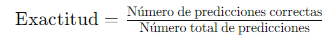
\includegraphics{images/EXACTITUD.png}
\item
  \textbf{Precisión (Precision):} Mide la proporción de verdaderos
  positivos sobre la suma de verdaderos positivos y falsos positivos.

  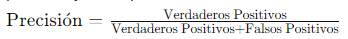
\includegraphics{images/Precision.png}
\item
  \textbf{Recall (Recuperación o Sensibilidad):} Mide la proporción de
  verdaderos positivos sobre la suma de verdaderos positivos y falsos
  negativos.

  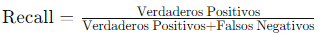
\includegraphics{images/Recall.png}
\item
  \textbf{F1-Score:} Es la media harmónica de precisión y recuperación.

  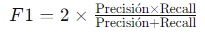
\includegraphics{images/F1.png}
\end{enumerate}

\hypertarget{clasificaciuxf3n-multiclase}{%
\subsubsection{\texorpdfstring{\textbf{Clasificación
Multiclase:}}{Clasificación Multiclase:}}\label{clasificaciuxf3n-multiclase}}

\begin{itemize}
\tightlist
\item
  Se pueden utilizar extensiones de las métricas de clasificación
  binaria, como la macro-precisión, la macro-recuperación y la
  micro-precisión.
\end{itemize}

\hypertarget{regresiuxf3n}{%
\subsubsection{\texorpdfstring{\textbf{Regresión:}}{Regresión:}}\label{regresiuxf3n}}

\begin{enumerate}
\def\labelenumi{\arabic{enumi}.}
\item
  \textbf{Error Cuadrático Medio (MSE):} Mide la media de los cuadrados
  de las diferencias entre las predicciones y los valores reales.

  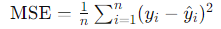
\includegraphics{images/Error cuadratico.png}
\item
  \textbf{Error Absoluto Medio (MAE):} Mide la media de las diferencias
  absolutas entre las predicciones y los valores reales.

  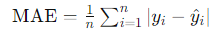
\includegraphics{images/Error absoluto.png}
\item
  \textbf{Coeficiente de Determinación} : Indica la proporción de la
  varianza en la variable dependiente que es predecible a partir de las
  variables independientes.

  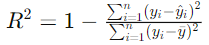
\includegraphics{images/Coeficiente de determinacion.png}
\end{enumerate}

Estas son solo algunas de las métricas de rendimiento comunes, y la
elección de la métrica adecuada depende de la naturaleza específica del
problema y los objetivos del modelo.

\hypertarget{regresiuxf3n-1}{%
\subsubsection{Regresión}\label{regresiuxf3n-1}}

Es un tipo de modelo utilizado para predecir valores numéricos basándose
en unos datos de entrada. La regresión busca establecer una relación
matemática entre las variables de entrada y una variable objetivo.

Algunos puntos clave sobre la regresión en el aprendizaje supervisado:

\begin{enumerate}
\def\labelenumi{\arabic{enumi}.}
\item
  \textbf{Objetivo Continuo:} A diferencia de la clasificación, donde el
  objetivo es predecir una etiqueta categórica, la regresión se utiliza
  cuando el objetivo es una variable continua. Por ejemplo, predecir el
  precio de una casa, la temperatura, o la cantidad de ventas.
\item
  \textbf{Modelo Matemático:} En este caso se busca encontrar la mejor
  función matemática que describa la relación entre las variables de
  entrada y la variable de salida. Este modelo puede ser lineal o no
  lineal, dependiendo de la naturaleza de los datos.
\item
  \textbf{Parámetros Ajustables:} Estos suelen tener parámetros
  ajustables que se modifican durante el entrenamiento del modelo para
  minimizar la diferencia entre las predicciones del modelo y los
  valores reales observados en los datos de entrenamiento.
\item
  \textbf{Evaluación del Rendimiento:} La calidad de un modelo de
  regresión se evalúa típicamente mediante métricas como el error
  cuadrático medio (MSE), el coeficiente de determinación (R-squared), o
  el error absoluto medio (MAE). Estas métricas cuantifican qué tan bien
  el modelo se ajusta a los datos observados.
\end{enumerate}

Ejemplos comunes de modelos de regresión incluyen la regresión lineal,
regresión polinómica, regresión de vecinos más cercanos (KNN), y
regresión de máquinas de soporte vectorial (SVR), entre otros.

\hypertarget{clasificaciuxf3n}{%
\subsubsection{Clasificación}\label{clasificaciuxf3n}}

El objetivo de la clasificación es asignar una etiqueta o categoría a un
conjunto de datos de entrada. Algunos datos importantes para entender la
clasificación son:

\begin{enumerate}
\def\labelenumi{\arabic{enumi}.}
\item
  \textbf{Objetivo Categórico:} La clasificación se utiliza cuando el
  resultado deseado es una etiqueta o categoría. Por ejemplo, determinar
  si un correo electrónico es spam o no spam, clasificar imágenes de
  dígitos escritos a mano en sus respectivos números, o predecir si un
  tumor es benigno o maligno.
\item
  \textbf{Modelo de Decisión:} Los modelos de clasificación buscan
  aprender una función que pueda tomar datos de entrada y asignarlos a
  categorías predefinidas. La salida del modelo es una etiqueta de
  clase.
\item
  \textbf{Aprendizaje de Patrones:} Durante el entrenamiento, el modelo
  analiza ejemplos de datos etiquetados para aprender patrones que
  puedan generalizarse a nuevas instancias.
\item
  \textbf{Evaluación del Rendimiento:} La calidad de un modelo de
  clasificación se evalúa mediante métricas como precisión, recall,
  F1-score, matriz de confusión y área bajo la curva ROC, entre otras.
  Estas métricas indican cómo de bien el modelo puede distinguir entre
  las clases.
\end{enumerate}

Ejemplos comunes de modelos de clasificación incluyen máquinas de
soporte vectorial (SVM), árboles de decisión, regresión logística, y
algoritmos de vecinos más cercanos (KNN), entre otros.

\hypertarget{metodologuxeda-1}{%
\subsection{Metodología}\label{metodologuxeda-1}}

El presente trabajo fue realizado para la materia Electiva tres del
programa de Ingenieria Biomedica, el docente nos suministro el paquete
\textbf{DynamicCancerDriverKM} el cual se encuentra en su GitHub.

\begin{enumerate}
\def\labelenumi{\arabic{enumi}.}
\tightlist
\item
  Antes de instalar cualquier paquete, es una buena práctica configurar
  un repositorio de CRAN.
\item
  Cargar paquete \textbf{\texttt{devtools}} en R es una herramienta útil
  para el desarrollo de paquetes, la instalación de paquetes
  directamente desde repositorios de GitHub, y la carga de paquetes que
  se encuentran en desarrollo o no están disponibles en el repositorio
  de CRAN
\item
  Instalar el codigo desde GitHub con devtools
\end{enumerate}

\textbf{Paso 1:} Primer Utiliza la función merge para combinar las
matrices BRCA\_normal y BRCA\_PT basándose en las columnas en comun, al
final pido que incluir todas las filas, tanto las que tienen
coincidencias como las que no.

\textbf{Paso 2:} Elimino las columas que no me interesan y dejo solo
genes y sample.

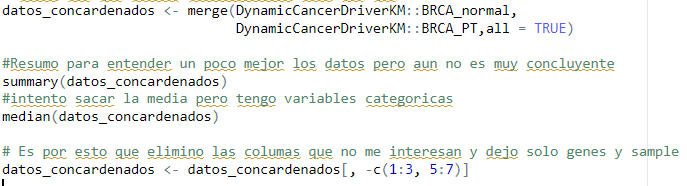
\includegraphics[width=4.79167in,height=\textheight]{images/PASO 1 Y 2.png}

\textbf{Paso 3:} Sacar el numero mas alto entre los datos, exclui a la
primera columna (sample) y multiplico por 0.00035 que es el 0.035\% , na
para excluir estos valores, con esto puedo revisar que genes estan
expresados calculo la media para tener un punto de partida y luego sacar
un valor, lo intente solo con la media aritmetica pero me enrrede, por
eso tuve que calcular un valor y multiplicar Tuve que volver a eliminar
sample\_type para refinar el dataframe

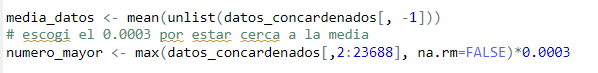
\includegraphics[width=3.90625in,height=\textheight]{images/3.png}

\textbf{\emph{Lo cargo como imagen ya que al colocar el codigo imprimia
tambien la salida lo que haria el documento muy extenso}}

\textbf{Paso 4:} Creo una copia donde pondre 1 a los datos que pasen el
umbral establecido y cero los que no. Utilice apply para que tome cada
columna x y utilice ifelse para asignar 1 si el valor es mayor que el
numero establecido como umbral

\textbf{Paso 5:} Limpie los datos el eliminar losgenes que no estan
expresados por lo menos en el 20\%

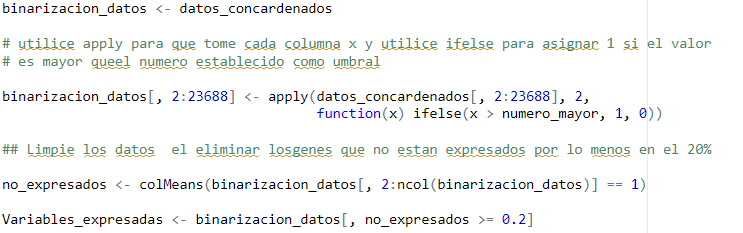
\includegraphics[width=3.875in,height=\textheight]{images/binarizacion.png}

\textbf{Paso 6:} Calcule las medias de cada columna de la matriz
booleana resultante, donde la media representa el porcentaje de unos en
cada columna.

\textbf{Paso 7:} renombre las variables para que concuerden respecto a
HGNC.symbol para poder concardenarlas y nuevamente para acceder por
columnas con colnames.

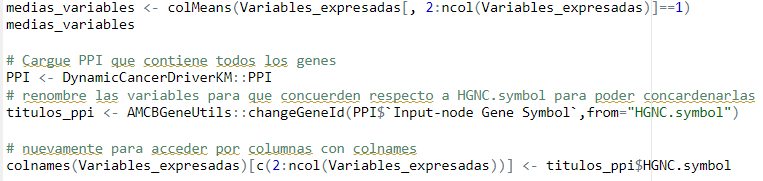
\includegraphics[width=4.29167in,height=\textheight]{images/MEDIAS.png}

\textbf{Paso 9:}

Luego con PPI \textbf{DynamicCancerDriverKM:: PPI} debia escoger los 100
genes principales con los grados de conexión más altos. Para esto fue
necesario lo siguiente:

\begin{enumerate}
\def\labelenumi{\arabic{enumi}.}
\tightlist
\item
  Agrupar los datos entre \textbf{\texttt{Input-node\ Gene\ Symbol}} y
  \textbf{\texttt{Output-node\ Gene\ Symbol} individualmente}
\item
  Con \textbf{\texttt{Summarise}} resumi los datos por agrupación y con
  la función \textbf{\texttt{n()}} solicito que cuente el numero de
  observaciones en cada grupo.
\item
  Asigné el resultado a una columna resultante llamada NN
\item
  Organice con \textbf{\texttt{Arrange}} los datos de manera descendente
  para lo que utilice \textbf{\texttt{(desc(NN))}}
\item
  Despues de tener ambos resultados organizados,
  \textbf{\texttt{Input-node\ Gene\ Symbol}} y
  \textbf{\texttt{Output-node\ Gene\ Symbol}} y como ambos tenian una
  segunda columna \textbf{NN} solo faltaba renombrar alguna de las
  columnas, bien sea en Input o Output, yo escogi Output y lo renombre
  igual que el otro grupo \textbf{\texttt{Input-node\ Gene\ Symbol}}
  para que al sumar se reconocieran los encabezados tanto de Agrupar
  como de Agrupar\_out.
\item
  Combiné ambos resultados en una sola matriz pero aun no estaban
  sumadas las veces que se repetia cada gen con
  \textbf{\texttt{bind\_rows}}.
\item
  Agrupé nuevamente los genes y las veces que se repiten
  \textbf{\texttt{group\_by}} y solicite el resumen con
  \textbf{\texttt{summarise}}
\end{enumerate}

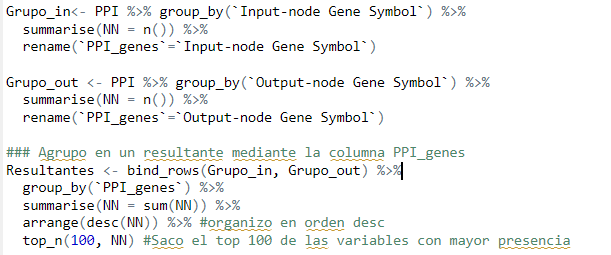
\includegraphics[width=4.63542in,height=\textheight]{images/GRUPOS.png}

\textbf{Paso 10:} CAMBIO LOS TITULOS EN FUNCION DE HGNC

\textbf{Paso 11:} Accedo a los titulos de cada variable genica y
Convertir los nombres de las variables en una matriz para unir con las
resultantes

\textbf{Paso 12:} Creo la interseccion entre matriz ppi y matriz
filtrada para empezar los modelos

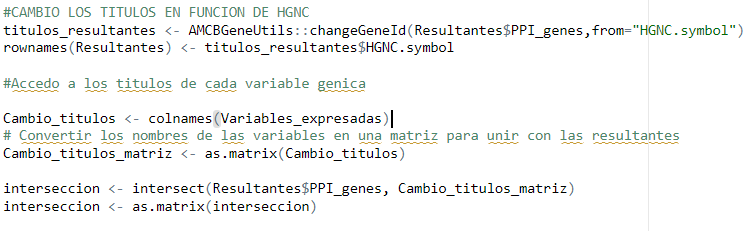
\includegraphics[width=4.55208in,height=\textheight]{images/titulos.png}

\textbf{Paso 13:} Establezco una semilla para garantizar la
reproducibilidad de los resultados cuando se generan números aleatorios.
Cada que ejecute el mismo código, obtengo los mismos resultados.

\includegraphics{}

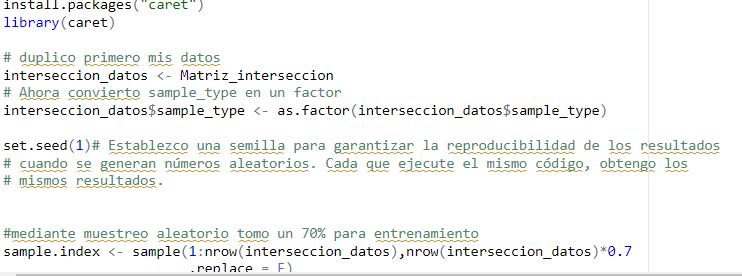
\includegraphics{images/knn1-01.png}

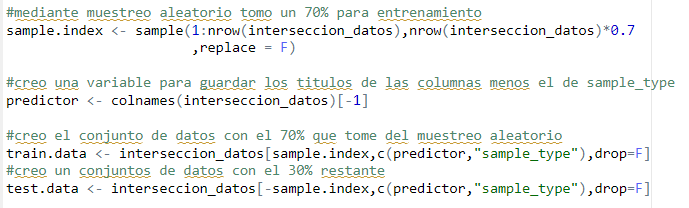
\includegraphics{images/knn2.png}

\textbf{Establezco control para el entrenamiento del modelo utilizando
validación cruzada con una proporción del 70\% para entrenamiento.}

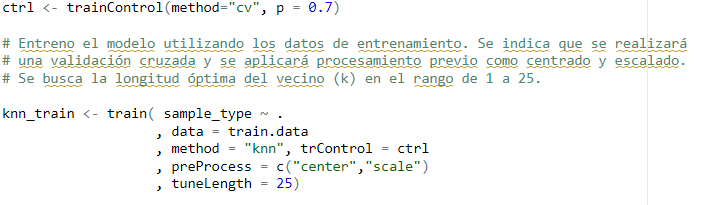
\includegraphics[width=5.72917in,height=\textheight]{images/knn3.png}

\textbf{Realiza predicciones en los datos de prueba utilizando el modelo
entrenado.}

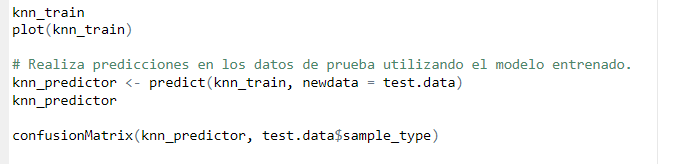
\includegraphics[width=5.38542in,height=\textheight]{images/knn4.png}

\hypertarget{retos-en-el-presente-trabajo}{%
\paragraph{Retos en el presente
trabajo}\label{retos-en-el-presente-trabajo}}

La mayor de las dificultades en el presente trabajo fue organizar los
datos antes de empezar con los modelos ya que eran demasiados datos y
organizar fue lo que mas me costo, adicional a la hora de hacer el
documento en rmakdown así compilara en el código a veces arrojaba error
por lo que para cumplir tuve que recurrir a cargar el
código~en~imágenes.

\hypertarget{conclusiones}{%
\subsubsection{Conclusiones}\label{conclusiones}}

Los modelos de prediccion pueden ser utilizados en multiples areas y es
responsabilidad del ingeniero prepararse en el desarrollo de muevas
estrategias de identificacion, procesamiento y desarrolo de una
enfermedad tan letal como el cancer. Con estos modelos no solo podemos
predecir cancer sino tambien muchas patologias mas.

\end{document}
